\section{Active and Nonlinear Mechanism Notes}

AMPA and NMDA synapses are opt-in extensions. NMDA includes a voltage-dependent magnesium block based on established reduced forms \citep{MayerWestbrookGuthrie1984,JahrStevens1990}. Na and delayed-rectifier K conductances follow Hodgkin-Huxley-style conductance-current logic \citep{HodgkinHuxley1952}. HCN, A-type K, and restrained calcium conductances are included as generic active-state stressors with provenance from dendritic physiology literature \citep{Magee1998,Magee1999,ConnorStevens1971,HuguenardMcCormick1992}.

These conductances are not cell-type-calibrated densities. They are disabled in the baseline reference configuration and should not be interpreted as fitted biological parameters. Their purpose in this manuscript is to test whether passive load-ratio conclusions survive nonlinear and active stress tests.

\begin{table}[!htbp]
\centering
\caption{\textbf{Active-extension parameter audit.} All mechanisms are disabled in the baseline reference configuration and enabled only through active-extension configurations or explicit protocols.}
\label{tab:active_parameters}
\resizebox{\textwidth}{!}{%
\begin{tabular}{lllll}
\toprule
Mechanism & Main parameters & Values & Units & Provenance/status \\
\midrule
AMPA & $g_{\max}$; $\tau_r$; $\tau_d$; $E_{\mathrm{rev}}$ & 1.4; 0.3; 3.0; 0 & nS; ms; ms; mV & active-extension double exponential \\
NMDA & $g_{\max}$; $\tau_r$; $\tau_d$; Mg; $\eta$; $\gamma$ & 0.7; 2.0; 80.0; 1.0; 3.57; 0.062 & nS; ms; ms; mM; mM; mV$^{-1}$ & reduced magnesium block family \\
Na & $\bar g$; $E_{\mathrm{rev}}$; gates & 6.0; 55; $m^3h$ & nS; mV; dimensionless & restrained HH-style extension \\
KDR & $\bar g$; $E_{\mathrm{rev}}$; gates & 1.5; -90; $n^4$ & nS; mV; dimensionless & restrained HH-style extension \\
HCN & $\bar g$; $E_{\mathrm{rev}}$; gates & 0.05; -30; $r$ & nS; mV; dimensionless & generic subthreshold HCN approximation \\
A-type K & $\bar g$; $E_{\mathrm{rev}}$; gates & 0.5; -90; $a^3b$ & nS; mV; dimensionless & restrained transient potassium extension \\
CaT & $\bar g$; $E_{\mathrm{rev}}$; gates & 0.05; 120; $p^2q$ & nS; mV; dimensionless & electrical-only restrained calcium extension \\
\bottomrule
\end{tabular}}
\end{table}


\begin{figure}[!htbp]
\centering
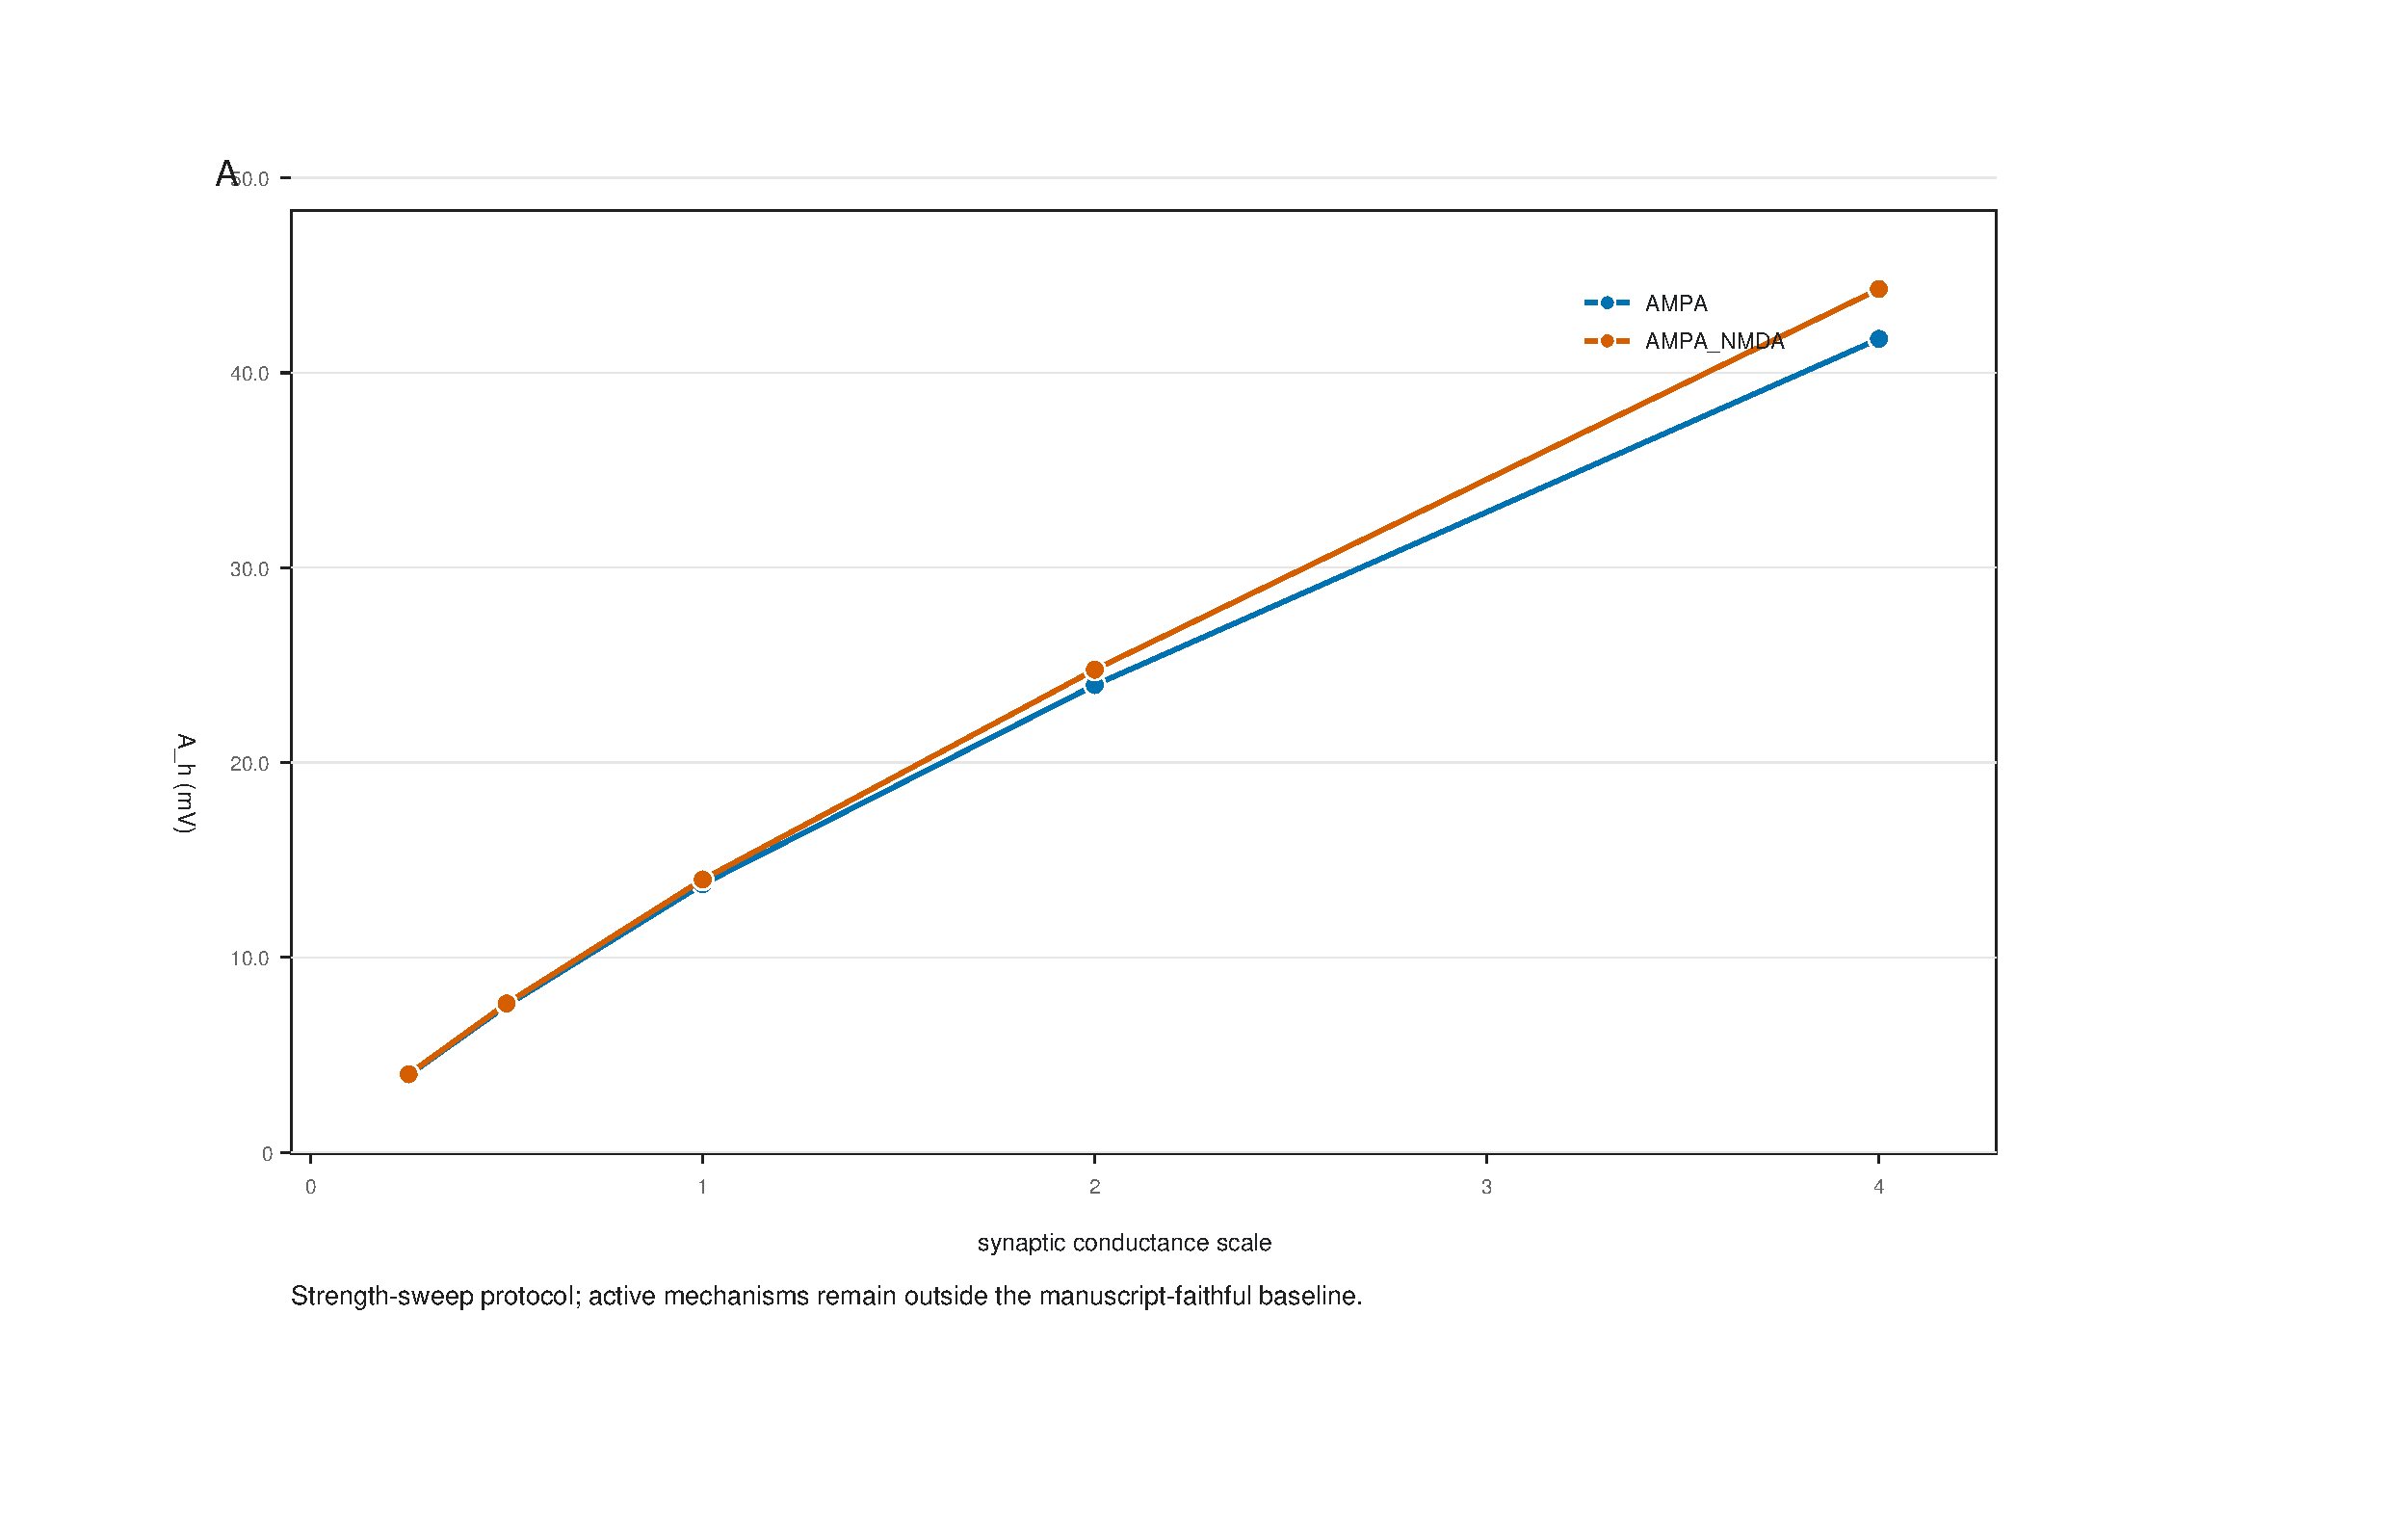
\includegraphics[width=0.85\textwidth,keepaspectratio]{../figures_publication/FigS6_active_protocol_strength.pdf}
\caption{\textbf{Figure S6.} Active AMPA and AMPA+NMDA strength-sweep protocol. The panel shows head-amplitude responses across pre-specified conductance scales for the active-extension protocol library.}
\label{fig:s6_active_strength}
\end{figure}

\begin{figure}[!htbp]
\centering
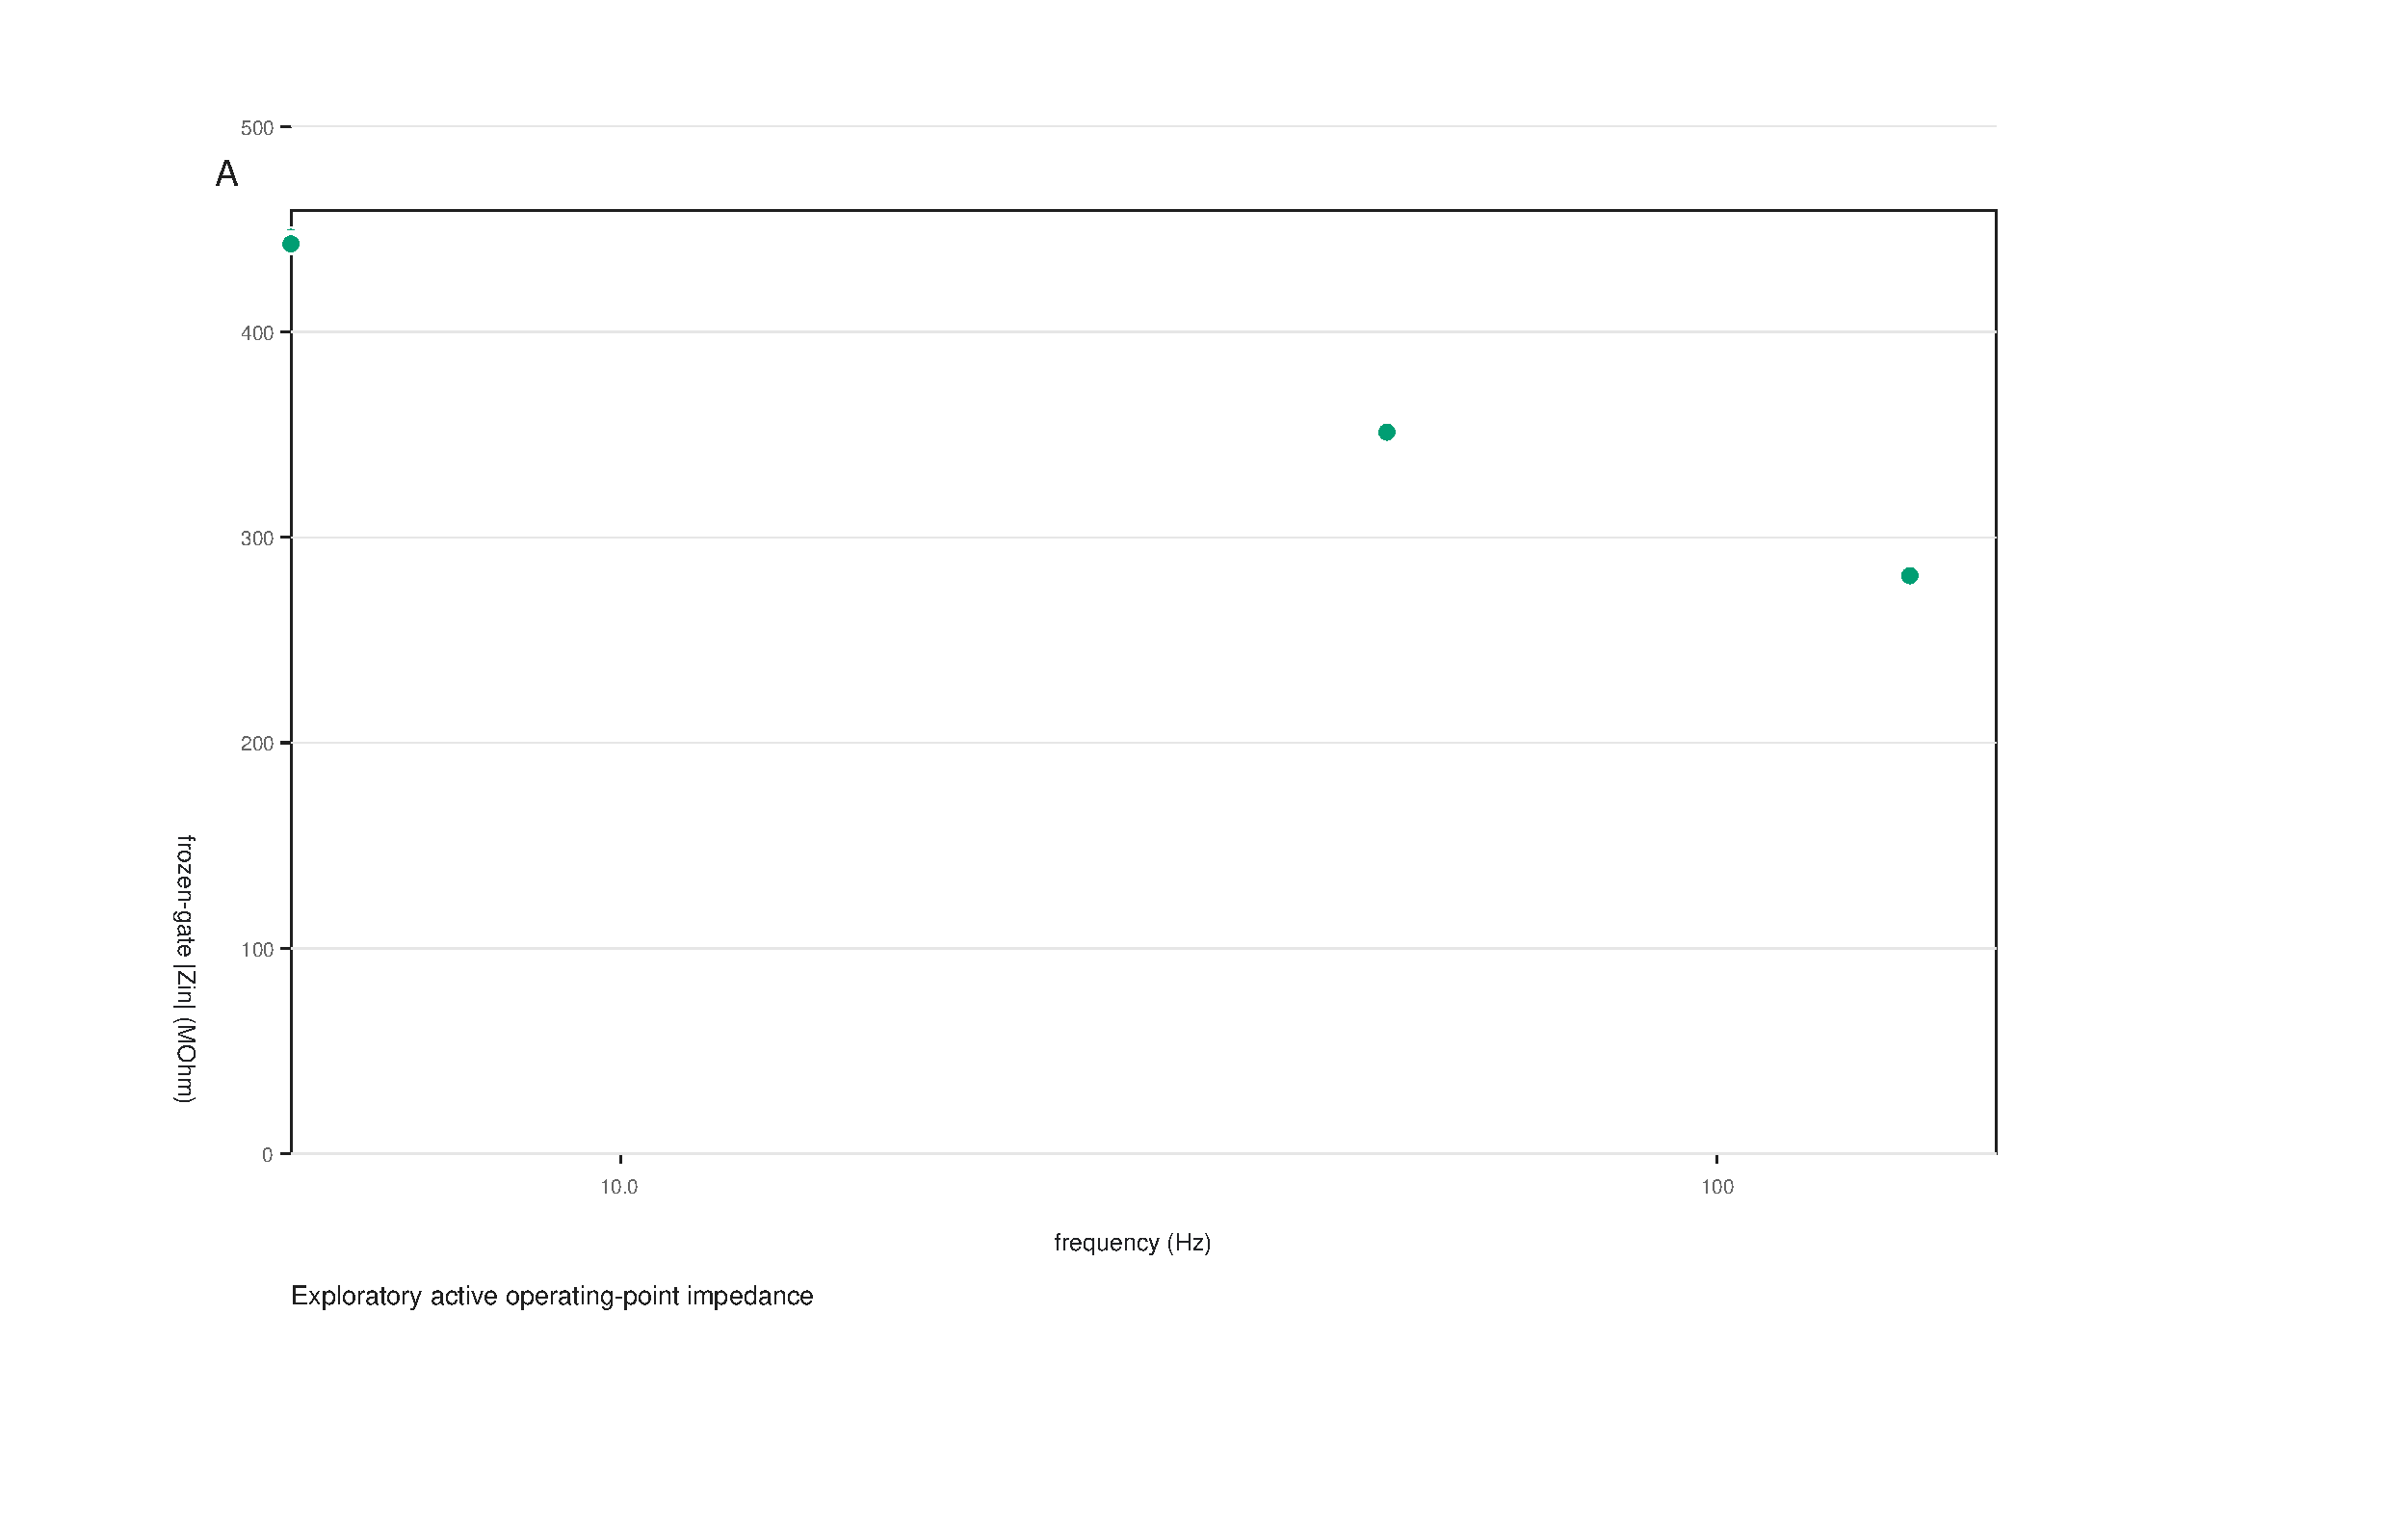
\includegraphics[width=0.85\textwidth,keepaspectratio]{../figures_publication/FigS7_active_impedance.pdf}
\caption{\textbf{Figure S7.} Exploratory frozen-gate operating-point impedance. The panel summarizes operating-point impedance estimates used as exploratory active-context descriptors.}
\label{fig:s7_active_impedance}
\end{figure}
